\chapter{绪论}\label{chap:introduction}{
\section{本文研究背景与意义}
随着信息技术迅猛发展,计算密集型任务与数据密集型任务已成为人工智能、流媒体、大数据、云计算和科学计算等领域面临的双重挑战。为应对这些挑战,并行系统架构在垂直扩展和水平扩展两个范式上不断发展。垂直扩展范式聚焦于单节点多核处理器(Multi-core CPUs)、异构加速器(如GPGPU、FPGA)等的深度协同优化,通过指令级或线程级并行提升计算能力;水平扩展范式则依赖于大规模分布式集群系统,结合松耦合任务调度与数据共享策略,实现跨节点的负载均衡与任务协作。

从并行编程的角度来看,这些范式基于以下并行模型:共享内存、消息传递和分布式共享内存(见图\ref{fig:model})。在共享内存模型中,所有计算核心共享一块全局主存,并通过各自私有的高速缓存(cache)来存储数据副本以加速数据访问。而在分布式集群环境中,各节点之间的物理内存彼此独立,通常采用消息传递模型和分布式共享内存模型。消息传递模型赋予集群中各节点上的进程独立的虚拟地址空间,进程间通过显式的通信原语(如 Send/Recv)完成数据交换。分布式共享内存模型则是共享内存模型在分布式系统上的扩展,将共享的理念从片上、节点内扩展到集群中,在物理上分离的内存之上构建一个虚拟共享内存抽象层,底层通过消息传递实现特定的迁移机制以完成数据共享。

上述三种模型中,分布式共享内存(Distributed Shared Memory, DSM)结合了共享内存与消息传递的优势,展现出以下核心特征:相较于消息传递,其采用透明的数据共享机制并保持与传统共享内存编程模型一致的抽象层,显著降低了分布式应用开发的复杂度;相较于多核共享内存架构,DSM 通过分布式扩展突破了单节点内存容量限制,在构建大规模负载处理系统时展现出更优的性价比。然而,DSM 仍面临两个关键挑战:昂贵的跨节点通信时延开销以及分布式环境下数据一致性维护的复杂性代价。

长期以来,由于这两个挑战以及单节点内多核处理器所展现的强大计算能力,分布式共享内存系统在大规模集群中的应用受到较大限制。但随着高性能网络互连和远程内存访问(RDMA)技术的不断进步,节点内与节点间通信性能差距正逐步缩小,分布式共享内存系统在计算与存储领域潜力正在重新受到关注。FaRM、Grappa、Argodsm、GAM、DRust 等基于 RDMA 高速网络的分布式共享内存系统层出不穷,它们通过低延迟、高带宽的远程内存访问,实现了更高效的数据共享和协同计算。这不仅有助于突破单节点内存容量的局限,还能在保证数据一致性的前提下,支持更大规模、更高并发的数据处理任务。

\begin{figure}[!htbp]
    \centering
    \begin{subfigure}[b]{0.35\textwidth}
      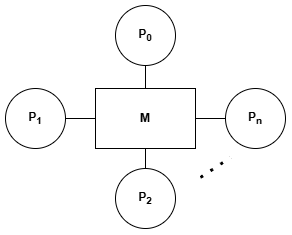
\includegraphics[width=\textwidth]{Img/multi-core.png}
      \caption{共享内存模型}
      \label{fig:multi-core}
    \end{subfigure}%
    \hspace{1.5cm}
    \begin{subfigure}[b]{0.35\textwidth}
      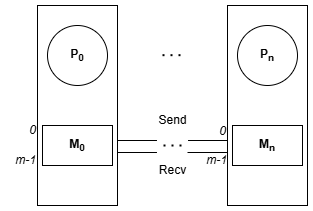
\includegraphics[width=\textwidth]{Img/message-passing.png}
      \caption{消息传递模型}
      \label{fig:message-passing}
    \end{subfigure}
    \begin{subfigure}[b]{0.6\textwidth}
      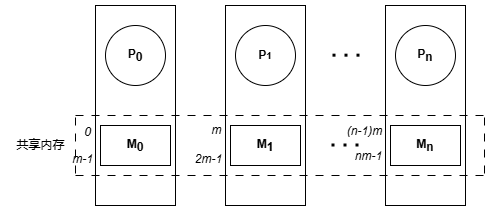
\includegraphics[width=\textwidth]{Img/dsm.png}
      \caption{分布式共享内存模型}
      \label{fig:dsm}
    \end{subfigure}
    \bicaption{并行编程模型}{Parallel programming model}
    \label{fig:model}
\end{figure}

研究支持 RDMA 通信的分布式共享内存系统,不仅为解决传统消息传递模型中显式数据分区和通信管理带来的复杂性提供了新思路,而且可为构建低延迟、高可扩展和高可靠的分布式系统奠定了坚实基础。通过这一技术融合,未来分布式系统可以在统一内存抽象下实现透明、高效的数据访问,同时兼顾计算密集型与数据密集型应用的需求,有助于推动新型分布式架构的发展和研究。

为避免重复造轮子,本文选择以国产软件分布式共享内存系统 JIAJIA\citep{huweiwu2001sma,huweiwu2024ca,1999huweiwuJIAJIA}  作为研究基础。JIAJIA由计算技术研究所胡伟武老师于上世纪 90 年代末设计,是我国首款自主研发的软件分布式共享内存系统,它以页为共享粒度,采用 NUMA 的内存组织结构(每个页有相应的家节点),在分布式的物理内存上构建了一个虚拟共享内存,并采用缓存机制来加速对远端内存访问。在数据一致性维护上,JIAJIA提出了与目录缓存一致性协议不同的基于锁的缓存一致性协议,该协议是域一致性模型的一种实现,使用锁而非目录来记录临界区域中所做的修改,避免了因目录条目维护而导致的复杂性和内存占用,大大增强了系统的可扩展性。JIAJIA 的问世对于国内和国际都是影响深远的,不仅填补了当时国内共享存储领域的研究空白,后续更被全球 20 多个国家和地区的 100 余家科研机构采用和研究,并且成功应用于国产高性能计算机。

分布式共享内存抽象建立在底层消息传递的基础之上,JIAJIA 底层采用传统单线程 UDP 通信来支持节点间通信。鉴于现代分布式集群系统普遍采用多核服务器并支持多网络协议栈通信,这一传统方案已无法充分利用现代化硬件资源与通信特性,JIAJIA 的性能可以通过利用 RDMA 和多线程来进一步优化。在JIAJIA基础之上设计实现 UDP 通信和 RDMA 通信双通信栈支持的 M-JIAJIA 既是解决传统软件 DSM 系统网络瓶颈的有效方案,也是探索软件分布式共享内存系统高性能网络下应用的基石。为充分利用底层硬件资源,M-JIAJIA将通信拆分为入队、发送、监听、接收和处理五阶段任务,利用多线程机制将通信流水线化,从而并行加速网络通信。在系统设计与实现过程中,为平衡可靠性、可扩展性以及易用性需求,始终秉持如下设计原则:
\begin{itemize}
    \item 正确性的优先级始终高于性能优化。
    \item 系统设计层次化、核心逻辑模块化,便于后续维护和扩展。
    \item 在不损害性能的前提下,尽可能增加系统易用性和灵活性。
\end{itemize}

\subsection{软件分布式共享内存系统概述}
在正式介绍软件分布式共享内存系统(下文简称为软件 DSM 系统)之前,有必要对分布式共享内存系统分类进行界定。根据节点间内存访问的耦合程序、一致性协议实现层级以及典型应用场景,分布式共享内存系统可以分为紧耦合(Tightly-Coupled)与松耦合(Loosely-Coupled)两类。紧耦合分布式共享内存系统以硬件为核心实现全局内存地址空间抽象,通常依赖于专用互连架构(如ccNUMA,NUCA)与定制缓存一致性协议(如MESI/MOESI),而松耦合分布式共享内存系统则是指在物理分散节点间构建逻辑统一的共享内存抽象的软件或轻量级硬件辅助实现。(如表~\ref{tab:dsm-different-implementations}所示)。

\begin{table}[!htbp]
    \bicaption{DSM的不同实现级别}{Different levels of DSM Implementation}% caption
    \label{tab:dsm-different-implementations}
    \centering
    \footnotesize% fontsize
    \setlength{\tabcolsep}{4pt}% column separation
    \renewcommand{\arraystretch}{1.5}% row space 
    \begin{tabular}{lcc}
        \hline
        DSM 实现级别 & 要求 & 示例\\
        \hline
        硬件 & 专用硬件(共享缓存、片上互连等)& ccNUMA、NUCA\\
        系统软件 & 操作系统虚拟管理机制修改 & IVY、Munin等 \\
         运行时用户库 & 基础通信能力 & TreadMarks、JIAJIA、OpenSHMEM 等\\
        语言或语言扩展 & 编译器支持 & PGAS语言(UPC、UPC++),OpenMP等 \\
        \hline
    \end{tabular}

    \vspace*{3ex}
    
    \begin{minipage}{\textwidth}% choose width suitably
	\mdseries\par\setlength\hangindent{2\ccwd} 表注:这里并不是严格划分,一些 DSM 的实现可能涉及多个层级协同实现。
    \end{minipage}
\end{table}

紧耦合分布式共享内存系统通常在单节点内实现,典型架构如多处理器之间的高速缓存一致非均匀内存访问(Cache Coherent Non-uniform memory access, ccNUMA)架构和多核之间的非均匀缓存访问(Non-uniform cache access, NUCA)架构。这些 DSM 的特点是支持低时延高带宽访存,由硬件自动维护全局内存状态以提供强一致性保证,以相对较小的缓存行(cacheline)为共享粒度,降低了发生假共享(false sharing)的概率。不足之处是构建成本高,过度依赖硬件而导致可扩展性和可移植性受限,而且共享内存的规模相对较小。

相比之下,属于松耦合范畴的软件 DSM 系统的实现则灵活的多,可以在系统软件(操作系统或编译器)、运行时库、语言等多个层次实现,具体区分可参见~\ref{sec:implementations}小结内容。
\subsection{软件分布式共享内存系统发展历程}
软件 DSM 系统的技术基础源于对操作系统虚拟内存机制和共享内存多处理器的研究。

虚拟内存机制通过内存管理单元(MMU)将虚拟地址映射到物理地址,并通过分段或分页机制结合换入/换出(swap in/out)为单个进程营造了一个巨大内存的假象。某种意义上,软件 DSM 系统可以看作是底层虚拟内存机制在分布式系统上的扩展,不过换入的数据来源和换出的目的地从传统的辅存变成了远端节点上的内存,这也是早期的软件 DSM 系统~\citep{likai1988ivy,bennett1990munin}依赖于修改操作系统的原因。而共享内存多处理器的研究为软件 DSM 系统提供了维护数据一致性的内存一致性模型,一致性模型是确保多处理器环境下正确读写共享数据的关键。

1986 年,Li Kai 博士在其论文\citep{likai1986svm}中验证了在分布式系统上构建共享虚拟内存系统的可行性,并实现了第一个软件 DSM 系统IVY\citep{likai1988ivy}。IVY 以页为粒度,支持单写多读(Single Writer Multiple Readers, SWMR)的数据访问模式,采用顺序一致性模型来保证数据一致性。这种设计使得并行程序在当时环境下取得了线性甚至超线性的加速,从而引发了大量对软件 DSM 的关注与研究。对软件 DSM 的研究热度持续了数十年,其中诞生了许多经典的软件 DSM 系统,如 Munin、TreadMarks、Midway、JIAJIA 等,不过这一热度随着多核处理器获得的巨大成功而逐渐减弱。

相比于 IVY,Munin~\citep{bennett1990munin}系统的最大特色是实现内存一致性的方案。为了降低维护分布式内存一致性所需的通信量以提升软件 DSM 系统的性能,它首次利用软件实现释放一致性(Release consistency),主张仅在特定的同步点才执行一致性操作。但 Munin 并非只采用了单个内存一致性模型,而是采用一种特定于数据类型的一致性模型,该模型通过识别用户对共享数据的注释以及编译器的提示来决定对每个对象使用何种一致性机制,允许开发者根据程序行为对一致性方法做动态决策。此外,为了解决 IVY 中出现的假共享问题(一个共享对象在处理器之间频繁移动),Munin 提出了多写协议与延迟更新机制,这种机制依赖于单节点上共享数据副本(copy)和其备份(twin)实现,多写协议允许不同处理器可以同时修改共享数据的不同部分(这种不同需要开发者保证),更新(diffs)通过逐字比较副本和备份产生,延迟更新是指更新的传播将延迟到处理器退出临界区域释放锁时,再将更新传播给所有包含修改的共享数据的副本的机器。

TreadMarks~\citep{amza1996treadmarks} 是另一个经典的软件 DSM 系统,它以线性字节数组的形式提供共享内存,为了进一步降低维护一致性导致的通信延迟对系统性能的影响,TreadMarks 采用懒惰更新释放一致性(Lazy release consistency)。与 Munin 采用的释放一致性(或称为急切更新释放一致性)不同的是,懒惰更新释放一致性发送的消息更少。在锁释放时,Munin 中释放锁的处理器会发送消息给所有拥有修改数据副本的其他处理器;而在懒惰更新释放一致性中,一致性消息仅在锁的最后一个释放者和新获取者之间传播。

JIAJIA 也是诞生于这一时期的国产软件 DSM 系统,不同于上述的一致性模型,JIAJIA 采用了域一致性模型(Scope consistency),这种一致性比懒惰更新释放一致性更宽松,将传播的修改的范围限制为锁保护的区域,即只有锁保护起来的区域中的修改才会传播给下一个锁获取者。不同于传统的基于目录的缓存一致性实现,JIAJIA 设计并采用了基于锁的缓存一致性协议方案,这种方案将锁关联的临界区域中产生的所有写通知(write notice)存储到锁中而非目录中,获取锁的处理器根据锁的写通知对其本地缓存数据副本进行失效或更新来保持缓存一致性。写通知呈现为修改的共享页的地址,即将修改的页的地址记录在锁关联的空间中。

进入本世纪以来的前十年,物理限制如功耗、互连延迟迫使处理器芯片从单核高频转向多核并行。这种架构变革使得传统分布式系统需要重新权衡网络通信成本与片内通信效率。相比于多核处理器通过共享缓存和片上网络降低片内通信开销,传统软件 DSM 系统依赖的网络通信成本要高几个数量级,这意味着想要传统软件 DSM 系统发挥以往的优势,并行程序在计算任务上所需的时间成本要比通信任务所需的时间成本高几个数量级,而且需要均衡的负载划分,这极大地限制了软件 DSM 的使用。受限的应用导致对软件DSM系统的研究的热度逐渐减退,对其研究也一直聚焦于一致性协议优化与减少通信次数~\citep{Cheung1999AMP, abe2003movinghomedsm}。

2014年,微软研究院推出 FaRM~\citep{drago2014farm}分布式共享内存平台,该工作首次将分布式共享内存与 RDMA 技术结合起来,使用 RDMA 网络协议栈替换传统 TCP/IP 网络协议栈,在降低消息传递延迟和增强吞吐上取得了不俗的性能表现。随后关于 RDMA 在分布式领域的研究层出不穷,DaRPC~\citep{stuedi2014DaRPC} 使用 RDMA 实现了一个异步非阻塞的超低延迟 RPC。FaSST~\citep{kalia2016fasst}尝试使用基于 RDMA 双向语义(Send/Recv)的RPCs构造高性能、可扩展的分布式事务处理系统。

Argodsm~\citep{kaxiras2015argodsm}面向无数据竞争程序,通过在本地做尽可能多的决策来避免因同步导致的长延迟。为达到这个目标,Argodsm 提出了一种新颖的缓存一致性协议和分层队列委托锁方案。该方案依靠自失效(self-invalidation)和自降级(self-downgrade)来实现缓存一致性协议。自失效意味着任何节点可以读取任何数据块,只要承诺在同步之前将缓存的副本主动无效化。自降级意味着一个节点可以自由地写入任何数据块,而无需从目录获得权限,只需在跨越同步点之前使其使写入对所有其他节点可见。自失效消除了新写入时的显式失效,意味着共享数据的家节点无需记录任何共享者;自降级消除了当读取未命中时为查找最新数据所需的目录间接寻址,相反,读未命中时,始终会在主节点找到正确的数据,这意味着完全不需要目录。这种设计和JIAJIA的基于锁的缓存一致性协议有异曲同工之处。同时,为了避免自失效引发未命中导致性能下降,系统提出分类目录来管理自失效,对数据进行分类以帮助节点筛选需要自失效的内容。在网络层,Argodsm 采用 MPI 底层通信机制。

Grappa~\citep{nelson2015grappa}针对数据密集型应用提供了一个延迟不敏感(latency-tolerant)的软件分布式共享内存系统,主张充分利用应用程序的并行性来解决以前 DSM 系统的不足,该系统将数据密集型计算框架 MapReduce、顶点为中心的图计算编程框架(vertex-cnetric)、关系查询引擎等映射到 DSM 上,利用多线程与高效的任务调度充分发挥底层硬件资源如核心、内存、网络的优势,在获得性能增益的同时降低了对此类框架编程的复杂度。不过尽管运行于 InfiniBand 网络之上,Grappa 并未原生支持 RDMA ,而是采用 MPI 作为底层消息库。

GAM~\citep{cai2018gam}是另一个利用 RDMA 技术的分布式共享内存平台,通过 Send/Recv 传递控制消息,RDMA Write 传递数据。平台遵循基于目录的缓存一致性,采用部分存储一致性模型(Partial Store Ordering, PSO),通过允许写入和后续的读取和写入重新排序,从而将写入从临界执行区域中移出。

Drust~\citep{haoranma2024drust} 认为尽管 RDMA 大幅降低了通信延迟,但与本地内存访问相比,远程访问产生的延迟仍高出几个数量级,为实现一致性所需的同步代价仍是导致 DSM 不实用的主要原因,因此主张运行时系统充分利用 Rust 编程语言中的所有权模型,该模型和单写多读的访问模式一致,通过自动限制读写顺序来简化一致性实现。

\subsection{软件分布式共享内存系统的机遇与挑战}
在新型硬件架构和应用场景变革的双重驱动下,现代软件分布式共享内存系统正迎来前所未有的机遇与挑战。

\textbf{机遇一:RDMA 高速网络。} RDMA 高速网络技术显著降低了跨节点访存开销,并呈现持续优化的趋势。根据InfiniBand 发布的带宽路线图,未来的 RDMA 网络链路带宽有望达到并超越Tbps级别。以英伟达 ConnecX 系列 RDMA 网卡为例:其目前最新产品 ConnnectX-8 超级网卡的最高带宽已达 800 Gbps。这种吞吐量接近本地内存访问速度,甚至优于某些 NUMA(非统一内存访问)节点间通信通道(例如 QPI)~\citep{cai2018gam}。这一进展和趋势极大缓解了传统软件 DSM 系统面临的高延迟通信瓶颈。

\textbf{机遇二:从计算到存储的应用场景转换。} 传统上,软件 DSM 系统主要用于并行计算,如科学模拟和数值计算,但随着多核处理器在并行处理性能上的优势日益凸显,软件 DSM 系统在该领域的应用受到严重挑战,目前仅适用于通信成本远小于计算成本的场景。不过随着大数据、人工智能和云计算等应用场景的迅猛发展,软件分布式共享内存系统的应用场景正在向支持大规模数据共享和存储的方向转变。基于分布式共享内存构建的键值存储、图计算及事务处理正成为软件 DSM 系统的新兴领域~\citep{nelson2015grappa}。

\textbf{关键挑战:强一致性与高性能之间的平衡。} 尽管高速网络技术大幅降低了传输延迟,但在软件 DSM 系统中实现严格的内存一致性(如顺序一致性)仍会引入不小的同步开销,从而对系统整体性能形成制约。如何在一致性维护与高性能运行之间找到最佳平衡,仍是当前软件分布式共享内存系统面临的关键挑战。

\section{本文研究内容与主要贡献}
本文对软件分布式共享内存系统


为开发人员提供了一个传统的类似多线程编程的共享内存抽象,极大的方便了分布式应用的开发与调试。

现代数据中心往往同时支持传统的以太网络和高性能的RDMA网络,尽管多数应用可以通过(IP over IB) IPoIB 的方式直接在RDMA 网络上运行,但这种方式被认为是
提供 RDMA 原生支持的通信栈旨在

针对上述,本文的主要贡献有:
1. 设计并实现了一个支持双通信栈(UDP+RDMA)的软件分布式共享内存系统 M-JIAJIA,其中采用多线程加速系统通信。

2. 设计并实现系统取页时远程预取机制,通过降低通信次数,大大提升了具有强局部性的应用程序的性能。

3. 深入分析了基于 \texttt{M-JIAJIA} 库的应用程序在各阶段的性能开销,并对 M-JIAJIA 与 OpenMPI 的关键接口进行了对比测试,从而为后续相关研究提供了重要的参考与支撑。

% 4. 利用 \texttt{M-JIAJIA} 设计实现了 \texttt{jacobi} 迭代算法,可用来在集群上进行线性方程组和热度扩散计算。
\section{本文组织结构}
本文的第一章介绍了文章的研究背景和意义,重点回顾了软件 DSM 系统的发展历程以及近年来相关技术演进趋势,指出了软件 DSM 系统现如今所面临的挑战与机遇,概述本文工作的研究内容和主要贡献。

第二章主要介绍工作所涉及的两个技术基础——软件分布式共享内存和RDMA,首先论述了软件 DSM 系统所涉及的关键技术,包括一致性模型、通信机制,介绍了几个经典和现代的软件 DSM 系统设计,并重点介绍了本文工作基础 JIAJIA 软件 DSM 系统的设计。最后介绍了 RDMA 技术的工作原理。

第三章主要介绍了M-JIAJIA的具体设计与实现,

第四章具体介绍了M-JIAJIA 的 RDMA 通信栈的设计与实现。

第五章主要介绍关于 M-JIAJIA 系统的性能分析与优化测试。首先介绍实验用到的程序,

第六章对本文的工作进行了总结,并展望 M-JIAJIA 系统后续可能的应用和研究方向。
}
